\documentclass{article}

% preambulo:
\usepackage[utf8]{inputenc}
% caracteres utf8 (tildes, enie) sin tener que usar comandos

\usepackage[spanish, es-tabla, es-nodecimaldot]{babel} 
% texto automatico en espaniol
% "tabla" en vez de "cuadro"
% no reemplaza puntos decimales por comas

%% NO AGREGAR PAQUETES ANTES DE ESTO, ES IMPORTANTE QUE BABEL ESTE PRIMERO

%%%%%%%%%%%%%%%%%%%%%%%%%%%%%%%%%
%% PAQUETES EXTRA %%%%%%%%%%%%%%%
%%%%%%%%%%%%%%%%%%%%%%%%%%%%%%%%%

\usepackage{subfiles}

\usepackage{amsmath} % PAQUETES DE MATEMATICA
\usepackage{amsfonts}
\usepackage{amssymb}


\usepackage{steinmetz} % comando \phase{}
\usepackage{units} % permite usar nicefrac
\usepackage{graphicx} % importar imagenes
\usepackage{float} % posicion H para floats
\usepackage[colorinlistoftodos]{todonotes}


\usepackage[a4paper, total={6in, 8in}]{geometry} 
% margenes correctos en subarchivos

\setlength{\parindent}{10pt}			%cuanta sangria al principio de un parrafo
\usepackage{indentfirst}				%pone sangria al primer parrafo de una seccion

\usepackage{listings}

%%%%%%%%%%%%%%%%%%%%%%%%%%%%%%%%%%%%%%%%%%%%%%%%%%%%%%%%%%%
%% NO AGREGAR PAQUETES DESPUES DE ESTO, ES IMPORTANTE QUE HYPERREF ESTE ULTIMO
\usepackage[hidelinks]{hyperref} % hipervinculos sin cajitas rojas




\begin{document}

\newgeometry{} % margenes default para la caratula
% caratula:
\begin{titlepage}
\newcommand{\HRule}{\rule{\linewidth}{0.5mm}}
\center
\mbox{\textsc{\LARGE \bfseries {Instituto Tecnol\'ogico de Buenos Aires}}}\\[1.5cm]
\textsc{\Large 22.99 Laboratorio de Microprocesadores}\\[0.5cm]


\HRule \\[0.6cm]
{ \Huge \bfseries Guía de Ejercicios N$^{\circ}$2: Introducción a Kinetis}\\[0.4cm] % Title of your document
\HRule \\[1.5cm]


{\large

\emph{Grupo 2}\\
\vspace{3px}

\begin{tabular}{lr} 	
\textsc{M\'aspero}, Martina  & 57120 \\
\textsc{Mestanza}, Joaqu\'in Mat\'ias  & 58288 \\
\textsc{Nowik}, Ariel Santiago  & 58309 \\
\textsc{Regueira}, Marcelo Daniel  & 58300 \\
\end{tabular}

\vspace{20px}

\emph{Profesores}\\
\vspace{3px}
\textsc{Jacoby}, Daniel Andr\'es\\ 	
\textsc{Magliola}, Nicol\'as\\ 	

\vspace{100px}

\begin{tabular}{ll}

Presentado: & 22/08/2019\\

\end{tabular}

}

\vfill

\end{titlepage}

% cambio los margenes para el resto del documento
\newgeometry{left=2.5cm, top=2.5cm, right=2cm, bottom=2cm}

% indice:
\tableofcontents
\newpage

\section*{Ejercicio 1 - Diagrama de Tiempos}
\addcontentsline{toc}{section}{Ejercicio 1 - Diagrama de Tiempos}

Se realizó el diagrama de tiempos correspondiente al siguiente código en assembler:

\begin{lstlisting}
org	$2000
ldaa	$C000
jmp	$2000
\end{lstlisting}

\begin{figure}[ht]
	\centering
	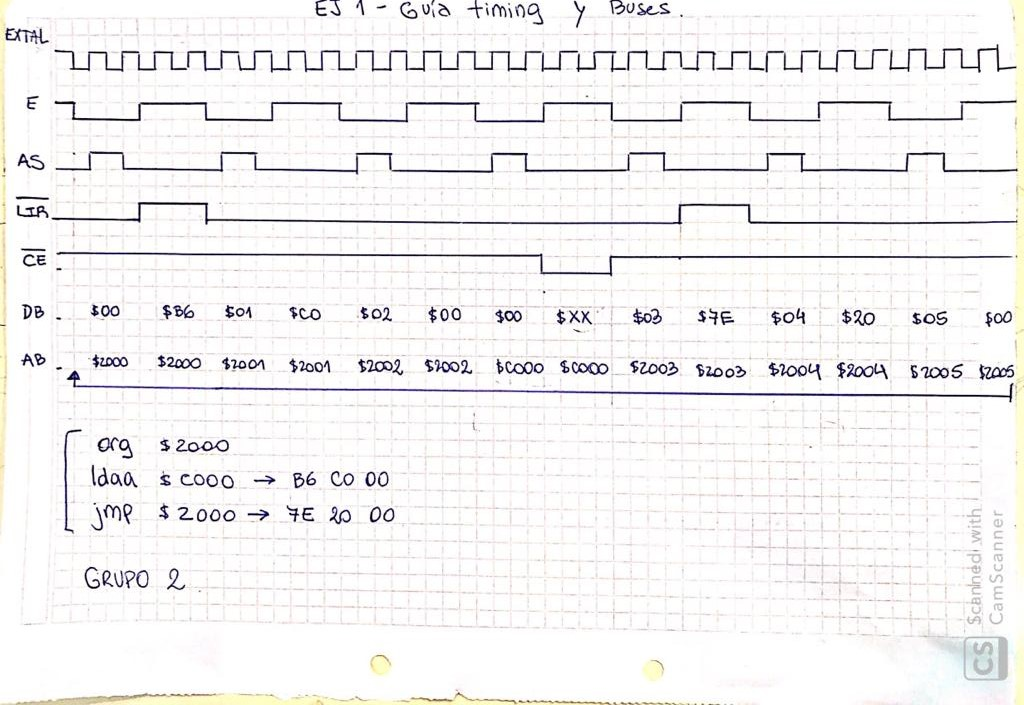
\includegraphics[width=0.8 \textwidth]
	{../Ej1/diagramaTiempos.jpeg}
	\caption{Diagrama de tiempos resultante}
	\label{fig:ej12}
\end{figure}

Cuando finaliza toda una vuelta, la flecha indica como continúa el código al iniciar una nueva.

\begin{figure}[ht]
	\centering
	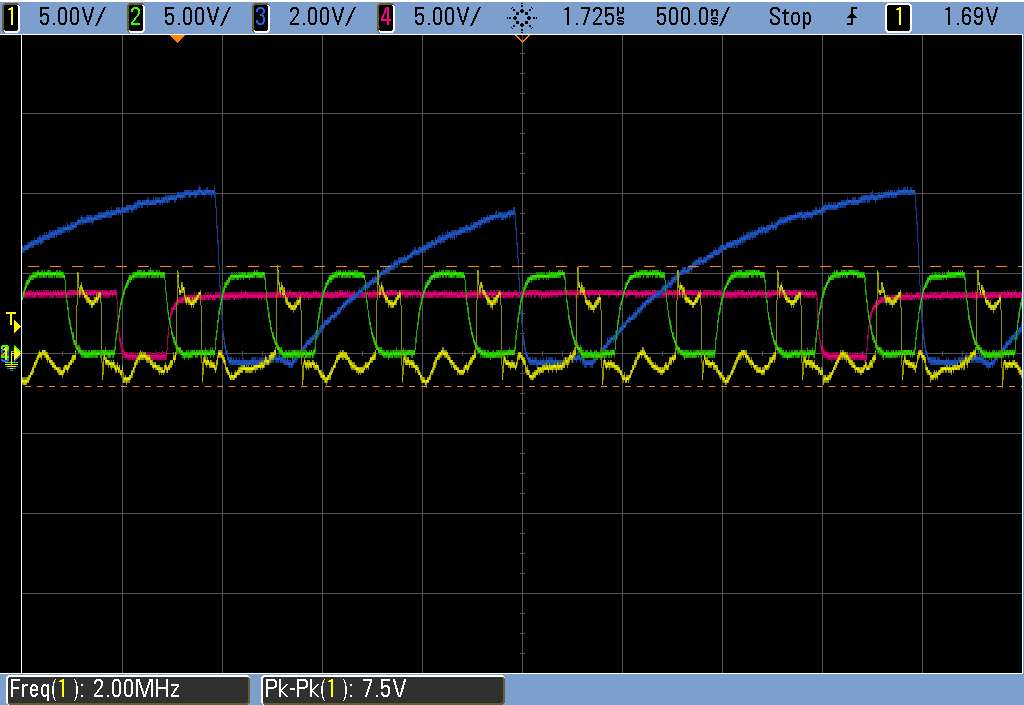
\includegraphics[width=0.7 \textwidth]
	{../Ej1/guia1_12.png}
	\caption{Señales características}
	\label{fig:ej12}
\end{figure}

En la captura anterior, la señal verde corresponde al E (data strobe), la amarilla es AS (address strobe), la azul es LIR (load instruction register), y la roja es el CE (chip enable).
Se pueden distinguir en que caso se da cada instrucción dado que una lleva más ciclos que la otra.
Cuando la señal de LIR baja a 0, es cuando viene una nueva instrucción. En el caso donde se observa que dura menos tiempo (3 ciclos), se corresponde a la instrucción jmp, dado que ésta requiere un ciclo para el opcode y dos más para la dirección de salto. El caso donde la señal de LIR dura más tiempo se corresponde con la instrucción ldaa, dado que requiere un ciclo más que la anterior para leer el dato solicitado en la posición \$C000.

\begin{figure}[ht]
	\centering
	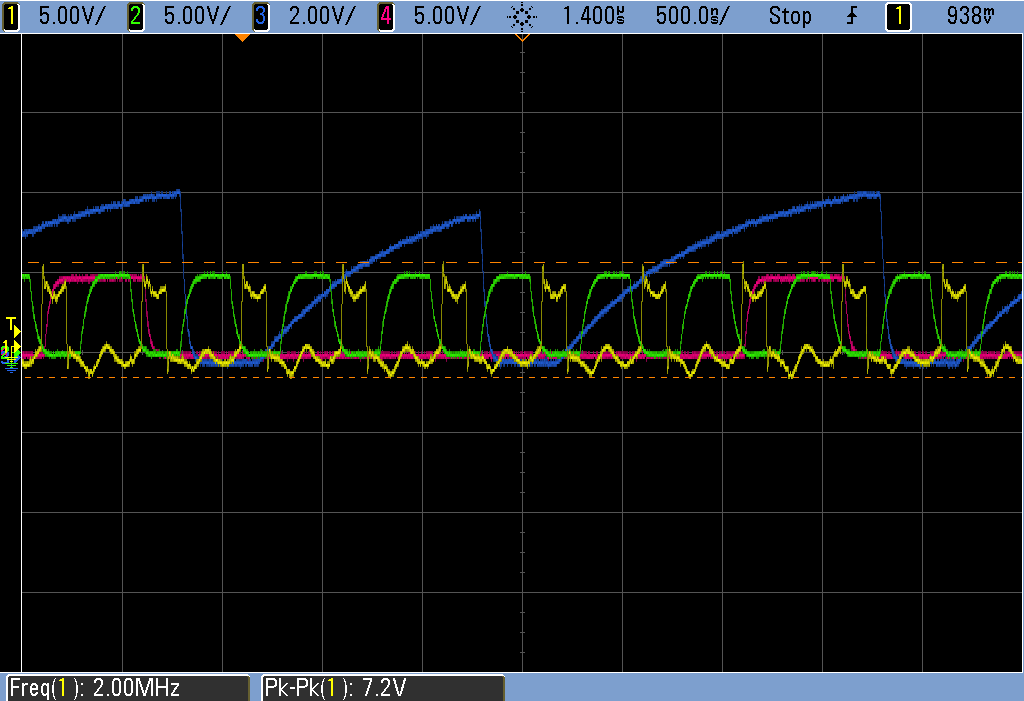
\includegraphics[width=0.7 \textwidth]
	{../Ej1/guia1_11.png}
	\caption{Señales características}
	\label{fig:ej11}
\end{figure}

En este caso, se tomo la misma medición, con la diferencia que la señal roja se corresponde con el bit más significativo del address bus, se puede ver como en el último ciclo de la instrucción ldaa, este pasa a ser 1, ya que es el momento en el que manda la dirección donde se encuentra el dato que se va a cargar en el registro A.

\newpage

\section*{Ejercicio 2 - Mapa de memoria}
\addcontentsline{toc}{section}{Ejercicio 2 - Mapa de memoria}

Realizando un \textit{dump} de la posición de memoria \$A000 se obtuvieron los siguientes resultados en el terminal:

\begin{figure}[ht]
	\centering
	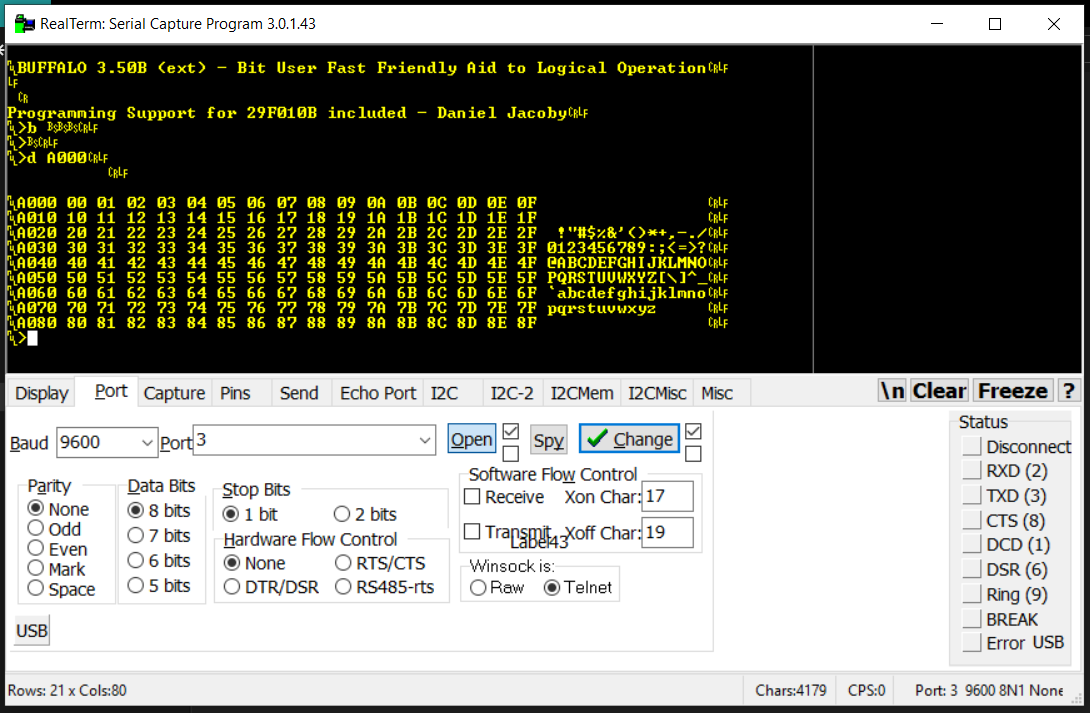
\includegraphics[width=0.8 \textwidth]
	{../Ej2/guia1_2.png}
	\caption{Resultado del dump en el terminal}
	\label{fig:ej2}
\end{figure}

Del mapa de memoria resultante se puede observar que, en cada posición desde la \$A000 hasta la \$A08F, los valores almacenados se corresponden directamente con los 8 bits menos significativos de cada dirección de memoria. Por ejemplo, la posición \$A012 posee el valor \$12. 

\newpage

\section*{Ejercicio 3 - Medición de tiempo de acceso}
\addcontentsline{toc}{section}{Ejercicio 3 - Medición de tiempo de acceso}

En este caso se buscó un método aproximado para medir el tiempo de acceso a la memoria FLASH. Para ello se utilizó una posición de memoria impar (\$C001) asegurándonos que tenga un valor par (\$10), de manera tal de poder observar la diferencia de tiempos entre las señales D0 del AS (address strobe) y el CE (chip enable) cuando cambian de estado. El código modificado para ello es el siguiente:

\begin{lstlisting}
org	$2000 
ldaa	$C001 (donde estaba el dato $10) 
jmp	$2000
\end{lstlisting}

\begin{figure}[ht]
	\centering
	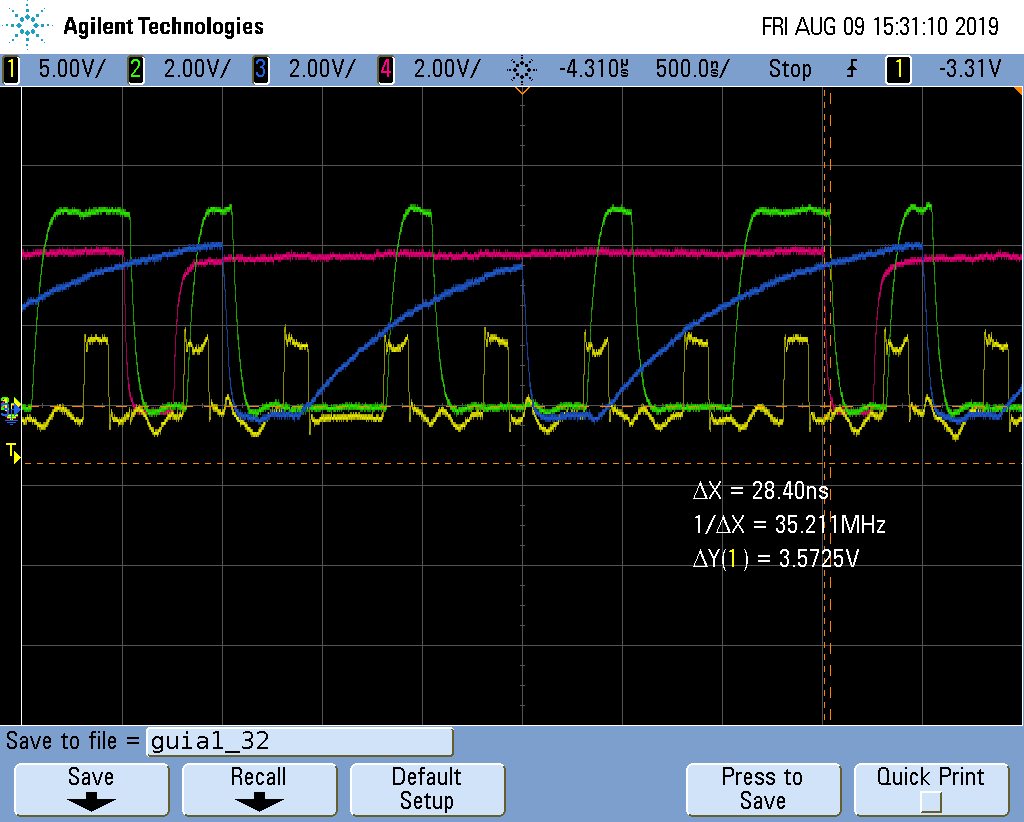
\includegraphics[width=0.8 \textwidth]
	{../Ej3/guia1_32.png}
	\caption{Medición de tiempos de acceso}
	\label{fig:ej2}
\end{figure}

En la captura tomada, la señal verde es el bit menos significativo del data bus (D0), la roja es el CE (chip enable), el AS es la amarilla (address strobe), y la azul es el LIR (load instruction register). 
Se midió el tiempo desde que la señal CE baja a 0 hasta que el D0 baja también a 0, que es el momento en que lee el dato. El tiempo resultante es de 28.4ns.


\end{document}
